\documentclass[11pt, A4]{article}
\usepackage[utf8]{inputenc}
\usepackage{tikz}
\usetikzlibrary{automata, positioning, arrows}

\title{Test Tikz}

\begin{document}

\begin{titlepage}
  \maketitle
\end{titlepage}

\begin{figure}[ht]
  \centering
  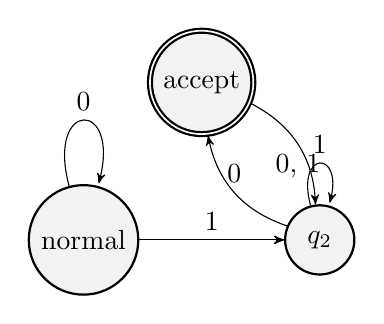
\begin{tikzpicture}
    % settings can be global or per picture
    \tikzset{
      ->,
      >=stealth',
      node distance=3cm,
      every state/.style={thick, fill=gray!10},
      initial text=$ $,
    }

    % states
    \node[state] (q1) {normal};
    \node[state, initial, right of=q1] (q2) {$q_2$};
    \node[state, accepting] at (1.5, 2) (q3) {accept};

    % transitions
    \draw (q1) edge[loop above] node{0} (q1)
          (q1) edge[above] node{1} (q2)
          (q2) edge[loop above] node{1} (q2)
          (q2) edge[bend left, above] node{0} (q3)
          (q3) edge[bend left, below] node{0, 1} (q2);

  \end{tikzpicture}
  \caption{Caption for the FSM}
  \label{fig:my_label}
\end{figure}


\end{document}
